%
% File acl2021.tex
%
%% Based on the style files for EMNLP 2020, which were
%% Based on the style files for ACL 2020, which were
%% Based on the style files for ACL 2018, NAACL 2018/19, which were
%% Based on the style files for ACL-2015, with some improvements
%%  taken from the NAACL-2016 style
%% Based on the style files for ACL-2014, which were, in turn,
%% based on ACL-2013, ACL-2012, ACL-2011, ACL-2010, ACL-IJCNLP-2009,
%% EACL-2009, IJCNLP-2008...
%% Based on the style files for EACL 2006 by 
%%e.agirre@ehu.es or Sergi.Balari@uab.es
%% and that of ACL 08 by Joakim Nivre and Noah Smith

\documentclass[11pt,a4paper]{article}
\usepackage[hyperref]{acl2021}

\usepackage[utf8]{inputenc}
\usepackage[T1]{fontenc}

\usepackage{times}
\usepackage{latexsym}
\renewcommand{\UrlFont}{\ttfamily\small}

% This is not strictly necessary, and may be commented out,
% but it will improve the layout of the manuscript,
% and will typically save some space.
\usepackage{microtype}

\usepackage{booktabs}
\usepackage{tabularx}
\newcolumntype{L}{>{\raggedright\arraybackslash}X}
\usepackage{svg}
\usepackage{multirow}
\usepackage{tikz}
\usepackage{amsmath}
\usepackage{natbib}
\usepackage{tabulary}

\usepackage{enumitem}
\newlist{lingex}{enumerate}{3} % easy numbering of examples
\setlist[lingex,1]{parsep=0pt,itemsep=1pt,label=(\arabic*),resume=lingexcount}
\newcommand\onelingex[1]{\begin{lingex}\item #1 \end{lingex}}
\usepackage{adjustbox}

\usepackage{textcomp}
\usepackage{amssymb}

%\aclfinalcopy % Uncomment this line for the final submission
%\def\aclpaperid{***} %  Enter the acl Paper ID here

%\setlength\titlebox{5cm}
% You can expand the titlebox if you need extra space
% to show all the authors. Please do not make the titlebox
% smaller than 5cm (the original size); we will check this
% in the camera-ready version and ask you to change it back.

\newcommand\BibTeX{B\textsc{ib}\TeX}

\title{Instructions for ACL-IJCNLP 2021 Proceedings}

\author{First Author \\
  Affiliation / Address line 1 \\
  Affiliation / Address line 2 \\
  Affiliation / Address line 3 \\
  \texttt{email@domain} \\\And
  Second Author \\
  Affiliation / Address line 1 \\
  Affiliation / Address line 2 \\
  Affiliation / Address line 3 \\
  \texttt{email@domain} \\}

\date{}

\begin{document}
\maketitle
\begin{abstract}
What we do: i) corpus study of laughter associated with dialogue acts and ii) testing the importance of laughter for DAR
\end{abstract}


\section{Introduction}

blah
% studies of laughter: humour, puns, functional role of laughter (Chiara), laughter prediction (Vlad)
% DAR and dialogue acts: why it is important
% gap: laughter was studied, but not when concerned with its co-locations with dialogue acts
% fill the gap:
% 1. we take a closer look, in which contexts laughter can occur w.r.t. DAs, this leads us to a hypothesis that laughter can be important for DAR
% 2. therefore, we look at laughter and its potential impact in DAR task
% 3. (we looks at non-verbals --- are they DAs?)

One important dialogical feature missing from text data is laughter,
which is ubiquitous in our everyday interactions.  We observe that in
the Switchboard dialogue corpus laughter comes about every 200 tokens.
Laughter also relates to the discourse structure of dialogue and can
relate to a \emph{laughable}, which can be an event or an entity in
the discourse (or external perceived event as well).  Laughter can
precede, follow or overlap the laughable, with the time alignment
between the laughter and laughable dependent on who produces the
laughable and the form of the laughter \citep{tian2016we}.  Laughter
can act as a contextual feature for determining the sincerity of an
utterance, e.g. when detecting sarcasm \citep{tepperman2006yeah}.

\section{Corpus study}
\label{sec:corpus}

In this section we analyse dialogue acts according to their co-location with
laughter and provide some qualitative insights from the
statistics. The distribution of laughs in different dialogue acts has
a rather uniform shape with a few outliers (Figure~\ref{fig:box-swda}). The
most distinct outlier is ``Nonverbal'' dialogue act which is
misleading with respect to laughter, because utterances only
containing a single laughter token fall into this category, however
they can serve, for example, to acknowledge a statement or to deflect
a question \citep{mazzocconi2019phd}.

\begin{figure}[htbp]
  \includesvg[width=\linewidth]{img/box-swda}
  \caption{Box plot for proportions of dialogue act which contain laughs.}
  \label{fig:box-swda}
\end{figure}

Let us introduce our comparison schema for the other two outliers,
Downplayer and Apology, comparing them with the most common dialogue
act in SWDA---Statement-Non-Opinion.  We take into consideration five
laughter-related dimensions of an utterance, and create 5-dimensional
representations of dialogue acts according to them. Each dimension's
value equals to the proportion of utterances of a given type which
contain laughter.
\begin{itemize}
\item[$\uparrow$] current utterance;
\item[$\nwarrow$] immediately preceding utterance by the same speaker;
\item[$\swarrow$] immediately preceding utterance by the other speaker;
\item[$\nearrow$] immediately following utterance by the same speaker;
\item[$\searrow$] immediately following utterance by the other speaker.
\end{itemize}

\begin{figure}[htbp]
  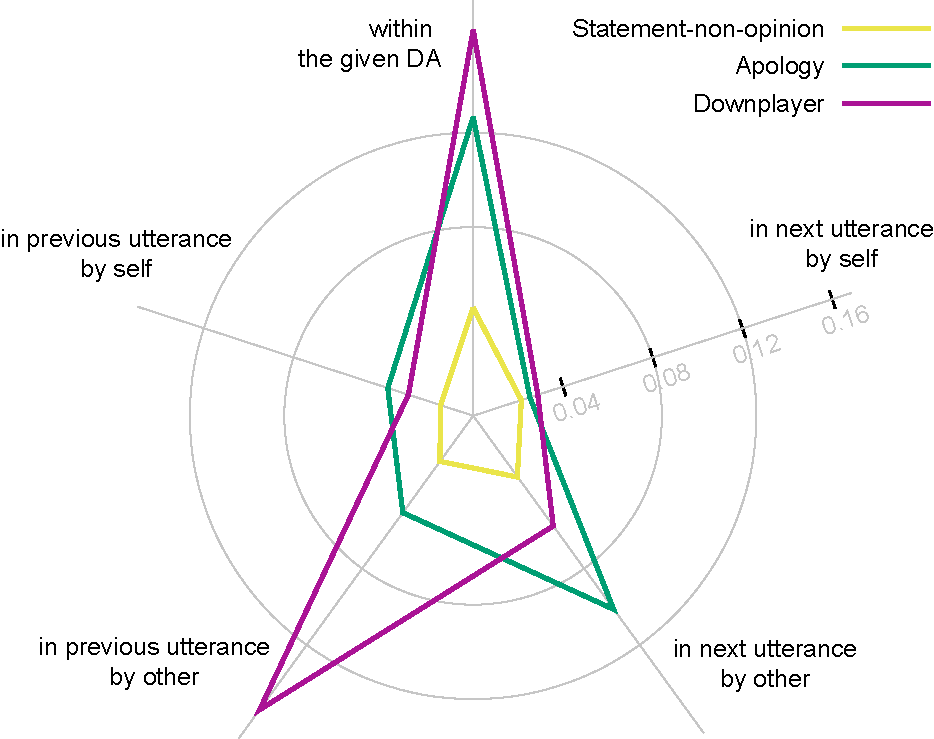
\includegraphics[width=\linewidth]{img/orbit-apology.pdf}
  \caption{Comparison of the most common dialogue act in
    SWDA---"Statement-Non-Opinion" (33.27\% of all utterances) with two
    outliers "Apology" (0.04\%) and "Downplayer" (0.05\%). Proportion
    of utterances which contain laughter are shown in association with
    each dialogue act. }
  \label{fig:orbit}
\end{figure}



For instance, \ref{ex:apology-downplayer} is an illustrative example
of the phenomenon shown on Figure \ref{fig:orbit}\footnote{Overlapping material is marked with hash signs.}. 
\begin{lingex}
\item\label{ex:apology-downplayer}
  \adjustbox{valign=t}{
    \begin{tabulary}{\linewidth}{>{\bf}lJ>{\em}R}
  A & I'm sorry to keep you waiting \#<laughter>.\# & Apology \\
  B & \#Okay\# <laughter>. / & Downplayer \\
  A & Uh, I was calling from work  & Statement (n/o) \\
    \end{tabulary}}
\end{lingex}


\section{Laughter’s role in dialogue act recognition}
\label{sec:dar}

% TODO motivation

\subsection{Data}\label{sec:data}
We perform experiments on the Switchboard Dialogue Act Corpus (SWDA), which is a subset of the larger Switchboard corpus, and the dialogue act-tagged portion of the AMI Meeting Corpus (AMI-DA). 
SWDA is tagged with a set of 220 dialogue act tags which, following  \citet{jurafskySwitchboardSWBDDAMSLShallowDiscourseFunction1997a}, we cluster into a smaller set of 42 tags.
AMI uses a smaller tagset of 16 dialogue acts \citep{GuidelinesDialogueAct2005}.

% TODO add laughter numbers for AMI!

\begin{table}[]
\centering
\begin{tabular}{@{}ll@{}}
\toprule
\textbf{Switchboard}       & \textbf{AMI Corpus}                     \\ \midrule
Dyadic                     & Multi-party                             \\
Casual conversation        & Mock business meeting                   \\
Telephone                  & In-person \& video                      \\ \midrule
English                    & English                                 \\ 
Native speakers            & Native \& non-native speakers           \\ 
early '90s                 & 2000s                                   \\ \midrule
2200 conversations         & 171 meetings                            \\
  \hspace{1em} 1155 in SWDA               & \hspace{1em} 139 in AMI-DA                           \\
400k utterances             & 118k utterances                         \\
3M tokens                  & 1.2M tokens                             \\ \bottomrule
\end{tabular}
  \caption{Comparison between Switchboard and the AMI Meeting Corpus}
  \label{table:corpora}
\end{table}

\paragraph{Preprocessing}
% - Preprocessing: remove disfluencies, acronyms and speaker tokens in AMI, removing laughter % Bill

We make an effort to normalize transcription conventions across SWDA and AMI.
We remove disfluency annotations and slashes from the end of utterances in SWDA.
In both corpora, acronyms are tokenized as individual letters. 
All utterances are lower-cased.

Utterances are tokenized using with a word piece tokenizer \citep{Wu2016} with a vocabulary of 30,000.
We add a special laughter token to the vocabulary and map all transcribed laughter to that token.
We also add five speaker tokens and prepend each utterance with a speaker token that uniquely identifies the corresponding speaker within that dialogue.


\subsection{Pre-training corpora}
We also experiment with three unlabeled dialogue corpora (Table~\ref{tab:pretraining-corpora}), which we use to provide further pre-training for the BERT encoder.

The first two corpora are constructed from the same source as the dialogue act corpora.
We use the SWDA portion of the un-labeled Switchboard corpus (SWBD) and the entire AMI corpus (including the 32 dialogues with no human-annotated DA tags that are not included in the DAR training set).
In both cases, we exclude dialogues that are reserved for DAR testing.

We also experiment with a much larger a corpus constructed from OpenSubtitles \citep{Lison2016}.
We used a manually constructed list of words frequenty used to refer to laughter in subtitles and replaced every occurance of one of these words with the special laughter token. 
Then, we collected every English-language subtitle file in which at least 1\% of the utterances contained laughter (about 11\% of the total).
Because utterances are not labeled with speaker in the OpenSubtitles corpus, we randomly assigned a speaker token to each utterance to maintain the format of the other dialouge corpora.

The pre-training corpora were prepared for the combined maksed language modeling and next sentence (utterance) prediction task, as described dy \citet{devlinBERTPretrainingDeep2018}.
For the smaller SWBD and AMI corpora, we generate and train on multiple epochs of data. Since there is randomness in the data preparation (e.g., which distrcactor sentences are chosen and which tokens are masked), we generate each training epoch separately.\footnote{For details, see the \href{https://github.com/huggingface/transformers/tree/1.1.0/examples/lm_finetuning}{finetuning example} from Hugging Face.}

\begin{table}[ht]
\centering
\begin{tabular}{@{}llll@{}}
\toprule
       & tokens & \% laughs & epochs\\ \midrule
AMI           & 1M     & 1.3             & 10     \\
SWBD          & 1.5M   & 0.5             & 10     \\
OpenSubtitles & 350M   & 0.3             & 1      \\ \bottomrule
\end{tabular}
\caption{Pre-training corpora, showing laughter representation as a percentage of total tokens and number of pre-training epochs generated.}\label{tab:pretraining-corpora}
\end{table}

\paragraph{}
Let us turn now to describing the neural network architectures that we used.

\subsection{The model}
\label{sec:model}
To test the effectiveness of BERT for DAR, we employ a simple neural architecture with two components: an encoder that vectorizes utterances, and a sequence model that predicts dialogue act tags from the vectorized utterances (Figure~\ref{fig:model-architecture}).
Since we are primarily interested in comparing different utterance encoders, we use a basic RNN as the sequence model in every configuration.\footnote{We have experimented with LSTM as the sequence model, but the accuracy was not significantly different compared to RNN. It can be explained by the absence of longer distance dependencies on this level of our model.} 
The RNN takes the encoded utterance as input at each time step,
and its hidden state is passed to a simple linear classification layer over dialogue act tags.
Conceptually, the encoded utterance represents the context-agnostic features of the utterance, and the hidden state of the RNN represents the full discourse context.

\begin{figure*}
  
\tikzstyle{rnn}=[rectangle,
  thick,
  minimum height=0.5cm,
  minimum width=2cm,
  fill=cyan]
\tikzstyle{encoder}=[rectangle,
  thick,
  minimum height=0.5cm,
  minimum width=2cm,
  fill=yellow]

\centering
\begin{tikzpicture}[>=latex,text height=1.5ex,text depth=0.25ex]
  \matrix[row sep=0.5cm,column sep=0.5cm] {
  % First line: Output labels
  \node (Y_0) []{$\hat{Y}_0$};&
  \node (Y_1) []{$\hat{Y}_1$};&
  \node (dots1) [] {$\dots$};  &
  \node (Y_T) []{$\hat{Y}_T$};&
  \\ % Second line: RNNs
  \node (RNN_0) [rnn]{RNN};&
  \node (RNN_1) [rnn]{RNN};&
  \node (dots2) [] {$\dots$};  &
  \node (RNN_T) [rnn]{RNN};&
  \\ % Third line: Linear layers
  \node (Encoder_0) [encoder]{Encoder};&
  \node (Encoder_1) [encoder]{Encoder};&
  \node (dots3) [] {$\dots$};  &
  \node (Encoder_T) [encoder]{Encoder};&
  \\ % Fourth line: Linear layers
  \node (Input_0) []{\small $ \underbrace{s^0,w^0_{0},w^0_{1},...,w^0_{n_0}}_{\text{Utterance 1}}$};&
  \node (Input_1) []{\small $ \underbrace{s^1,w^1_{0},w^1_{1},...,w^1_{n_1}}_{\text{Utterance 2}}$};&
  \node (dots4) [] {$\dots$};  &
  \node (Input_T) []{\small $ \underbrace{s^T,w^T_{0},w^T_{1},...,w^T_{n_T}}_{\text{Utterance T}}$};&
  \\ };
  \path[->]
  (Input_0) edge[thick]  (Encoder_0)	
  (Input_1) edge[thick] (Encoder_1)	
  (Input_T) edge[thick] (Encoder_T)	

  (Encoder_0) edge[thick] node[right] {} (RNN_0)	
  (Encoder_1) edge[thick] node[right] {} (RNN_1)	
  (Encoder_T) edge[thick] node[right] {} (RNN_T)	

  (RNN_0) edge[thick] (Y_0)	
  (RNN_1) edge[thick] (Y_1)	
  (RNN_T) edge[thick] (Y_T)	

  (RNN_0) edge[thick] node[above] {$h_1$} (RNN_1)
  (RNN_1) edge[thick] node[above] {$h_2$} (dots2)
  (dots2) edge[thick] node[above] {$h_T$} (RNN_T)
  ;
\end{tikzpicture}

  \caption{Simple neural dialogue act recognition sequence model}
  \label{fig:model-architecture}
\end{figure*}

As a baseline utterance encoder, we use a word-level CNN with window sizes of 3, 4, and 5, each with 100 feature maps \citep{kimConvolutionalNeuralNetworks2014}. 
The model uses 100-dimensional word embeddings, which are initialized with pre-trained gloVe vectors \citep{penningtonGloveGlobalVectors2014}.

For the BERT utterance encoder, we use the BERT\textsubscript{BASE} model with hidden size of 768 and 12 transformer layers and self-attention heads \citep[][\S3.1]{devlinBERTPretrainingDeep2018}.
In our implementation, we use the un-cased model provided by \citet{wolfHuggingFaceTransformersStateoftheart2019}.

The next section will introduce the experiments that we have carried out and will discuss the results that we obtained from them.

\subsection{Experiment 1: Impact of laughter} \label{sec:experiment1}   % Vlad
In the first experiment we investigated whether laughter, as an example of a dialogue-specific signal, is a helpful feature for DAR.
Therefore, we train another version of each model: one that containing laughs (\texttt{L}) and one with laughs left out (\texttt{NL}), and compare their performances in DAR task.
Table~\ref{table:laughter-total-acc} compares the results from applying the models with two different utterance encoders (\texttt{BERT}, \texttt{CNN}).

First of all, we can see that the \texttt{BERT} utterance encoder outperforms \texttt{CNN} in all the cases.
From observing the effect of laughters, we can see differences in performance depending on the dialogue act, regardless how often laughter occurs in the current or adjacent utterances (see Figure~\ref{fig:by-da} in Appendix~\ref{sec:suppl}).
The strongest evidence for laughter as a helpful feature was found in SWDA for the \texttt{BERT} utterance encoder, where macro-F1 score increases by 7.89 percentage points.

\begin{table}
  \centering
  \begin{tabular}{@{}lcccc@{}}
    \toprule
                      & \multicolumn{2}{c}{SWDA} & \multicolumn{2}{c}{AMI-DA} \\ \midrule
                      & F1    & acc.  & F1    & acc.       \\ 
    \texttt{BERT-NL}  & 38.10 & 77.07 & 49.09 & 67.06       \\ 
    \texttt{BERT-L}   & 45.99 & 76.93 & 50.17 & 67.12       \\ \midrule
    \texttt{CNN-NL}   & 37.23 & 75.08 & 38.37 & 63.46        \\
    \texttt{CNN-L}    & 27.59 & 75.40 & 37.94 & 64.30        \\ \midrule
    Majority class    & 0.78  & 33.56 &  1.88 & 28.27      \\ \bottomrule
    
  \end{tabular}
  \caption{Comparison of macro-average F1 and accuracy depending on using laughter on the training phase. }
  \label{table:laughter-total-acc}
\end{table}

Confusion matrices (Figure~\ref{fig:swda-cm}) provide some food for thought. Most of the misclassifications fall into the majority classes, such as \emph{sd} (Statement-non-opinion), in the left edge of the matrix. However, there are some important exceptions, such as \emph{rhetorical questions}, that are misclassified as other forms of questions due to their surface question-like form.
Importantly, laughter helps to classify rhetorical questions correctly, this is because in a conversation it can be used as a device to cancel seriousness or sincerity \citep{ginzburg2015understanding,tepperman2006yeah}, in this case, of a question.
Therefore, questions, like the one we show in the example in Table~\ref{table:example-qh}, are easier to disambiguate with the help of laughter.
\begin{table}
      \small
  \centering
  \begin{tabularx}{\linewidth}{llL}
    \toprule
    Speaker & DA & Utterance \\ \midrule
        \multicolumn{3}{c}{\emph{(Talking about hobbies)}}\\
    B   & sd	&  Um, as far as spare time, they talked about, \\
    B	& \% & I don't, + I think, \\
    B	& qh & who has any spare time \texttt{<laughter>}? \\
    A	& x & \texttt{<laughter>}.\\
             \bottomrule
  \end{tabularx}
  \caption{Example from the SWDA corpus (sw3735). B's contribution \emph{qh} (Rhetorical question) is misinterpreted as \emph{qw} (Wh-question) by the BERT model without laughs in training data. }
  \label{table:example-qh}
\end{table}



  \begin{figure}
  \centering
  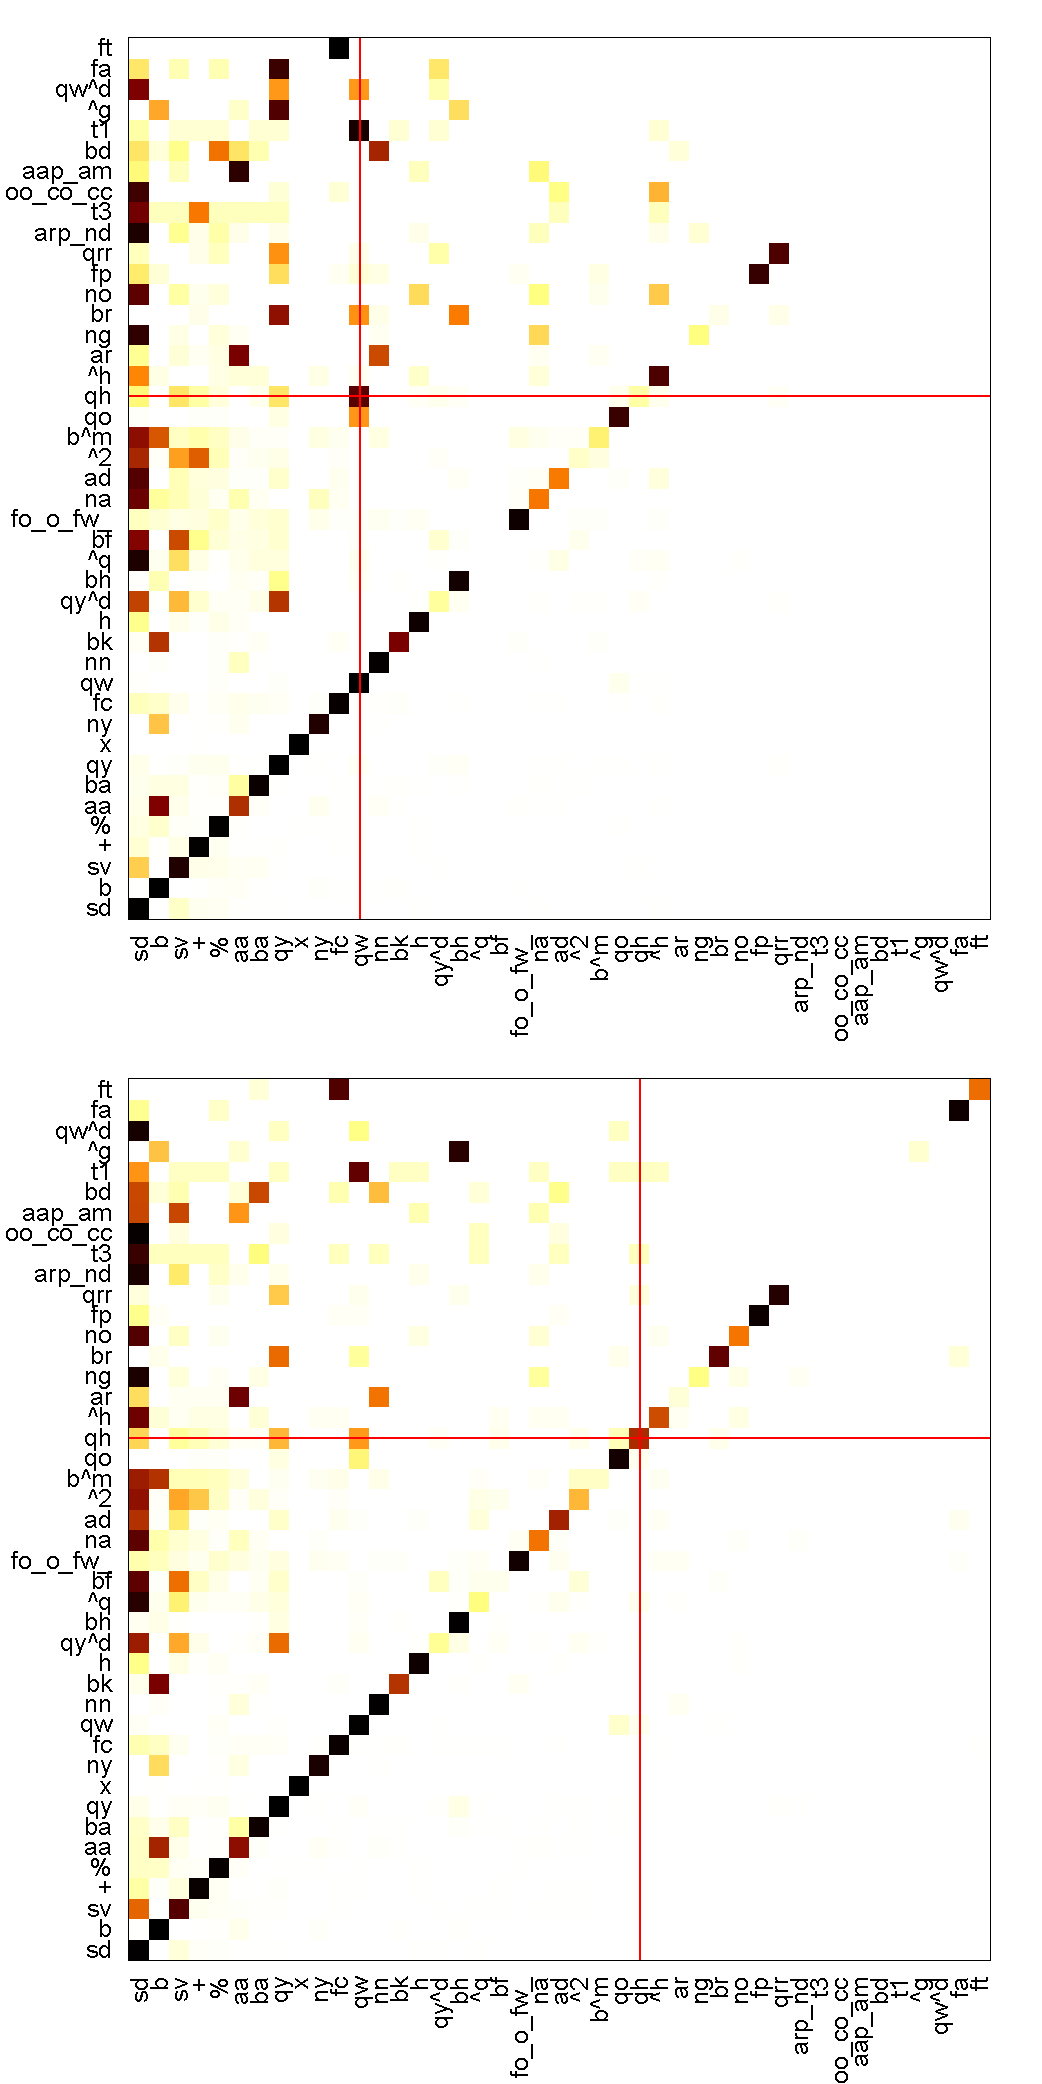
\includegraphics[width=1.0\linewidth]{img/swda-cm.pdf}
  \caption{Confusion matrices for \texttt{BERT-NL} (top) vs \texttt{BERT-L} (bottom); SWDA corpus. Solid line shows the improvement in classification of rhetorical questions.}
    \label{fig:swda-cm}
  \end{figure}


  % TODO: mapping groups?

\section{Experiment 2: laughter and pre-training}
\label{sec:exper-2:-laught}
% what if we additionally pre-train on dialogue corpora? With laughters... will it help?

\section{Laughter as a non-verbal dialogue act}
\label{sec:laughter-as-non}



\section{Discussion}
On the question of laughter impact, this study found that laughter is more helpful in SWDA corpus than in AMI-DA.
Due to the nature of interactions over the phone, SWDA dialogue participants can not rely on visual signals, such as gestures and facial expressions.
Our results support the hypothesis that in SWDA, vocalizations such as laughter are more pronounced and therefore more helpful in disambiguating dialogue acts.

This may also explain why all our best models perform better on SWDA: more of the information that interlocutors and dialogue act annotators rely on is present SWDA transcripts, whereas AMI-DA annotators receive clear instructions to pay attention to the videos \citep{GuidelinesDialogueAct2005}.
This finding is consistent with that of \citet{bavelas2008gesturing} who demonstrate that in face-to-face dialogue, visual components, such as gestures, can convey information that is independent from what is conveyed by speech.

There is abundant room for further progress in determining how other speech-related information, such as prosody and disfluencies, can be incorporated into the DAR model.
\citet{stolckeDialogueActModeling2000} showed that dialogue acts can have specific prosodic manifestations that can be used to improve dialogue act classification.
Furthermore, in relation to laughter, its form (duration, arousal level) can be informative about its function and position w.r.t. to laughable \citep{tian2016we,mazzocconi2019phd}.
Incorporating such information is crucial if models pre-trained on large-scale text corpora are to be adapted for use in dialogue applications.

\section*{Acknowledgments}

The acknowledgments should go immediately before the references. Do not number the acknowledgments section.
\textbf{Do not include this section when submitting your paper for review.}

\bibliographystyle{acl_natbib}
\bibliography{semdial}
\appendix
\onecolumn
\section{Supplementary materials}\label{sec:suppl}

\begin{figure*}[h!]
  \centering
  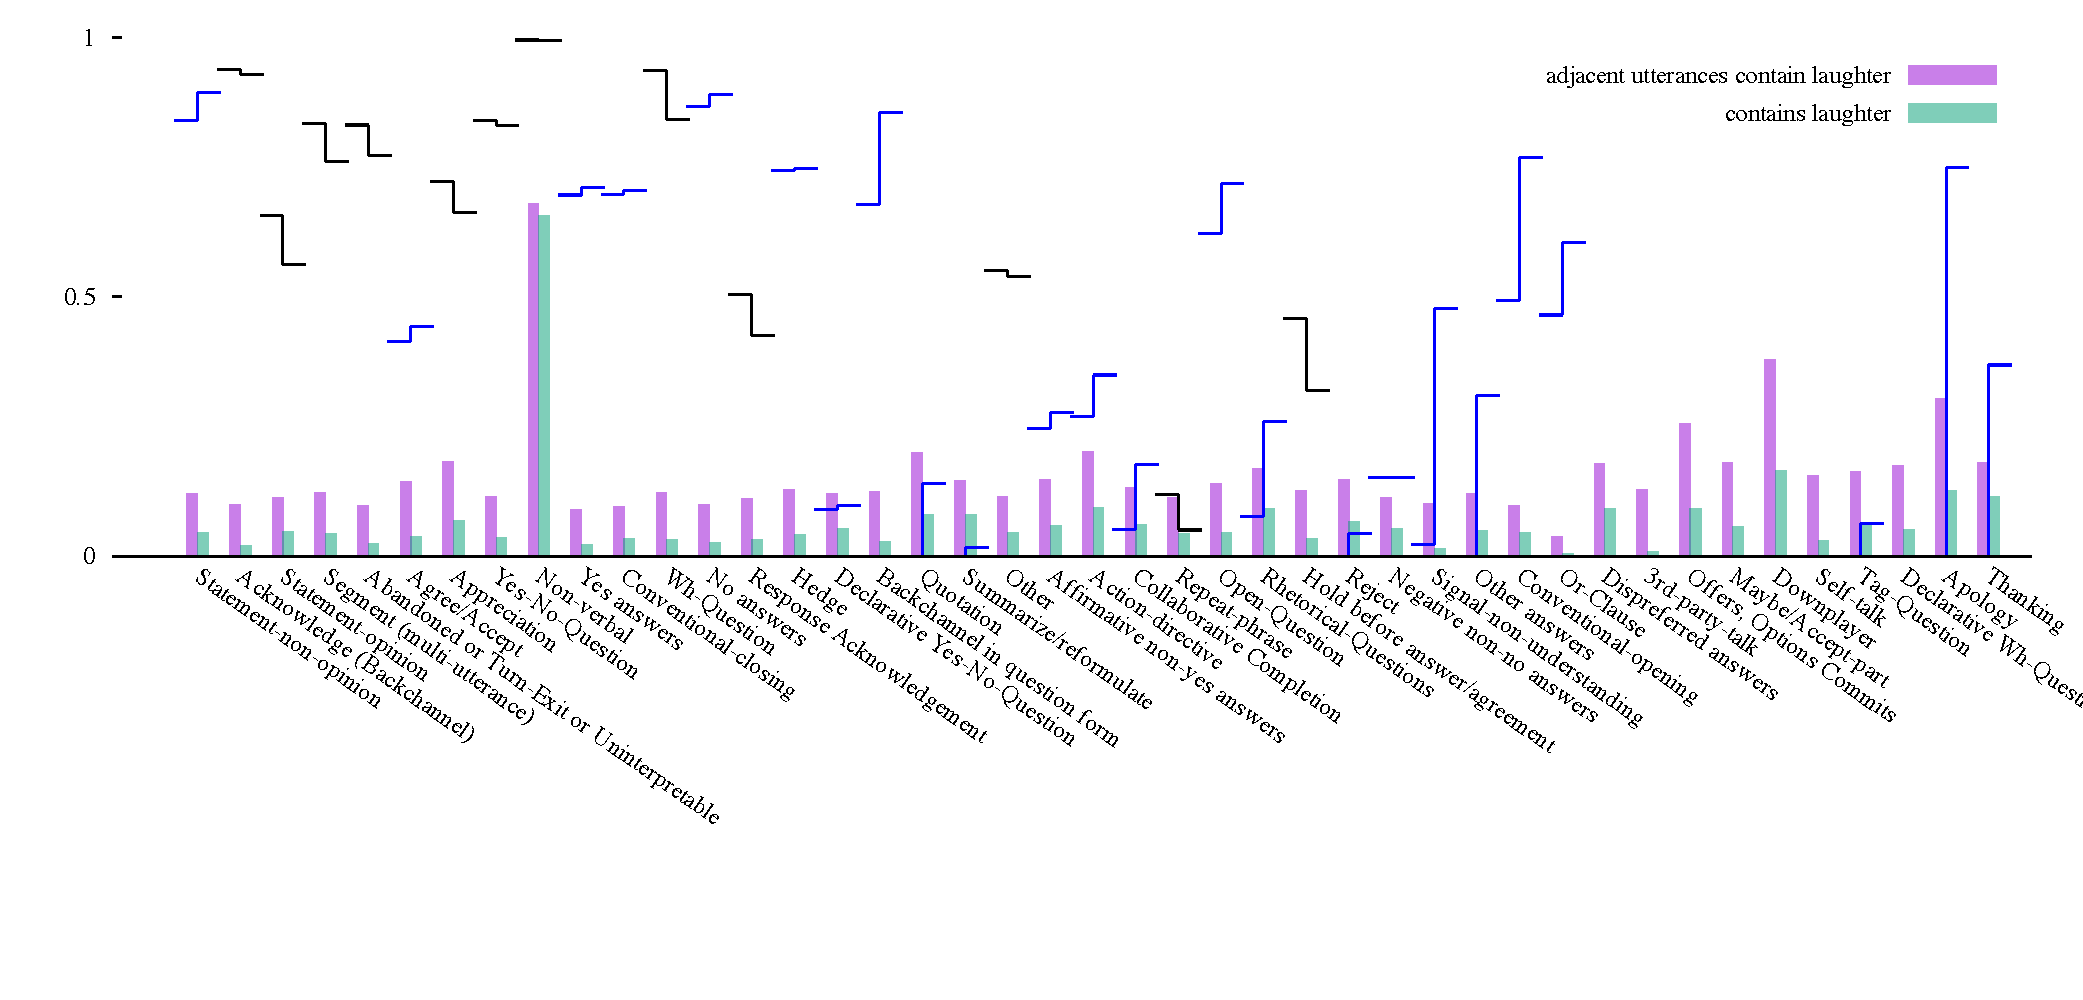
\includegraphics[width=\linewidth]{img/SWDA-bertLvsNL.pdf}
  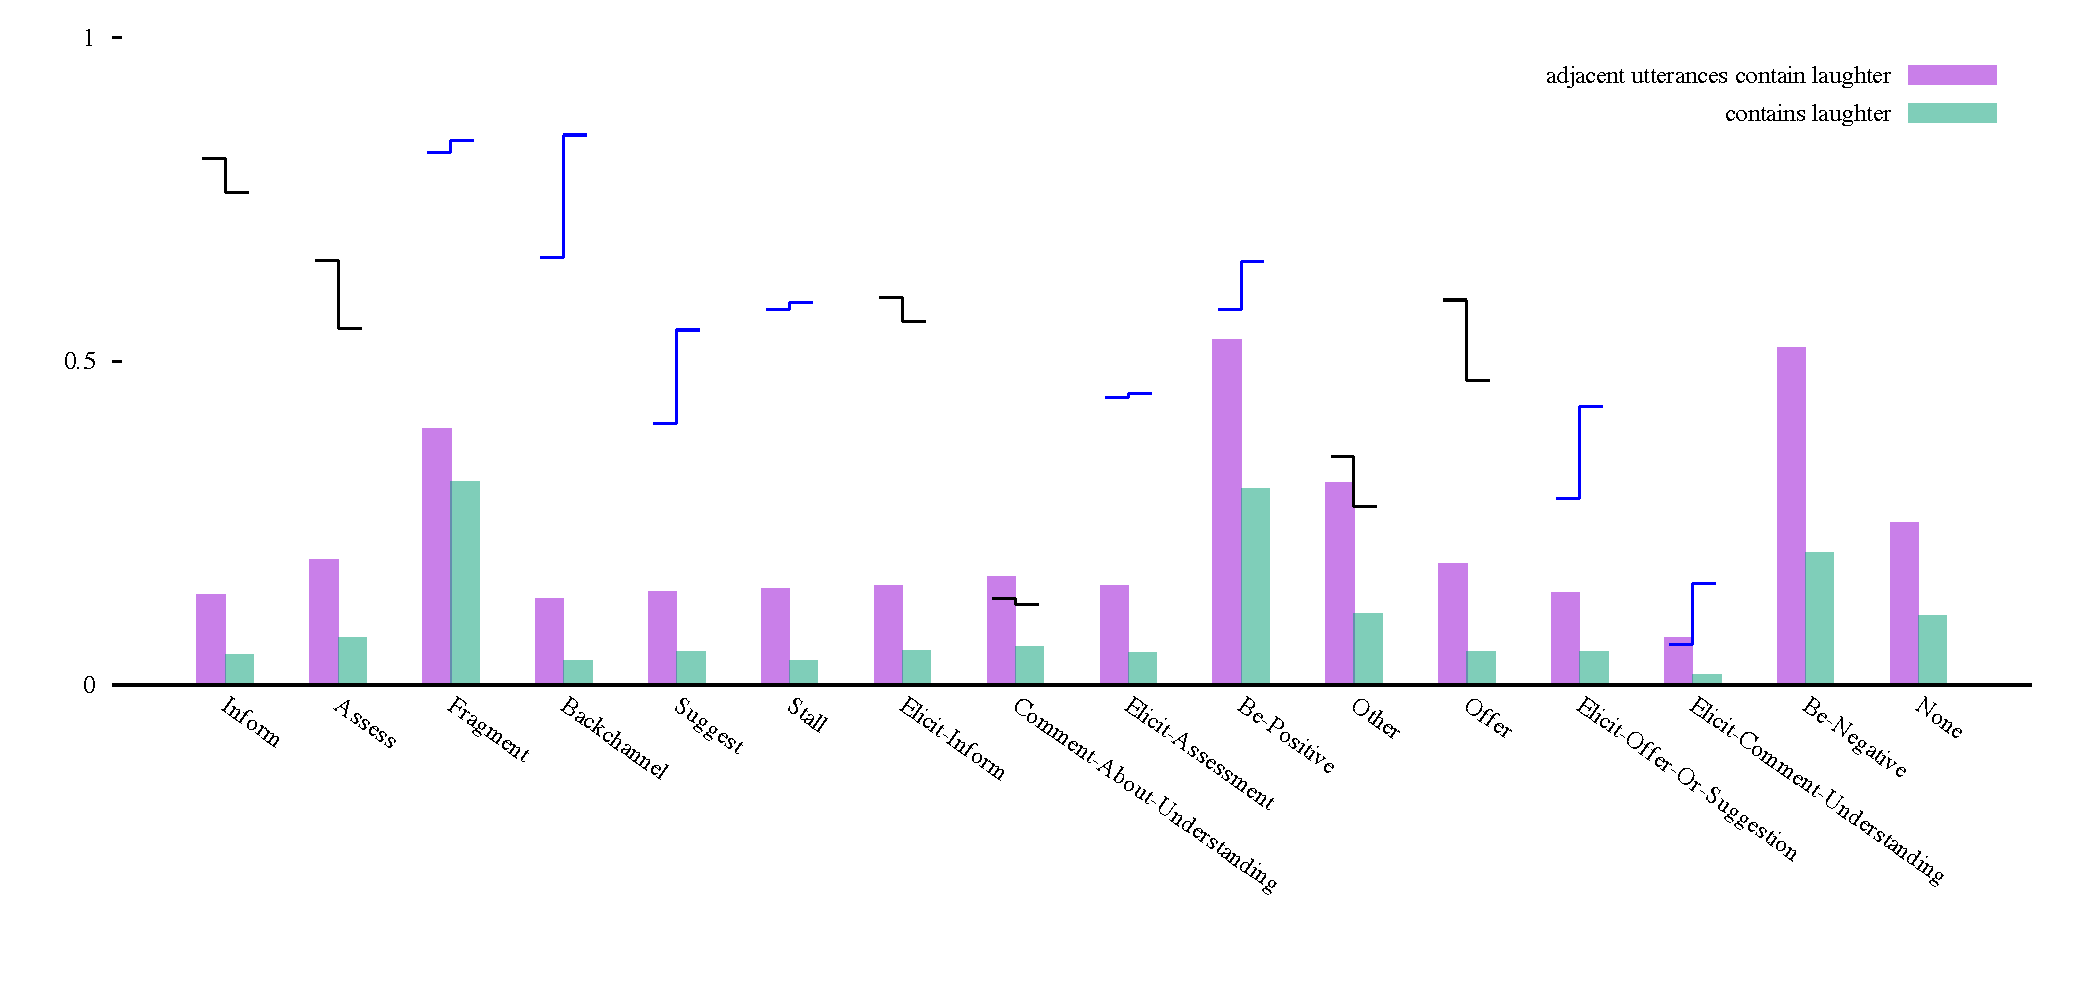
\includegraphics[width=\linewidth]{img/AMI-DA-bertLvsNL.pdf}
  \caption{Change in accuracy for each dialogue act (\texttt{BERT-NL} vs \texttt{BERT-L}). Positive changes when adding laughter (\texttt{BERT-L}) are shown in blue. Vertical bars indicate how often dialogue act is associated with laughter. Top chart: SWDA, Bottom chart: AMI-DA. }
    \label{fig:by-da}
\end{figure*}

\begin{figure*}[h!]
  \centering
  \fontsize{8}{10}\selectfont
  \includesvg[width=\linewidth]{img/da-svd-verbal}
  \caption{}
    \label{fig:da-svd}
\end{figure*}

\end{document}
